% ===================================================================================================
\chapter{Results}
% ===================================================================================================

% ----------------------------------------------------------------------------------
\section{Vacancies}
% ----------------------------------------------------------------------------------
In Fig. \ref{Fig:1Vac_results} and \ref{Fig:2Vac_results} we can see the number of T and H atoms bound to the mono- and divacancies as a function of time, for different temperatures. 
For comparison, the results of the monoisotopic, 'vacuum annealing', simulations are also shown. 
We can see that at all three temperatures, tritium-removal occurs at a higher rate when isotope exchange is involved.
While the difference is more prominent at lower temperatures, it is noticeable also at 500 K, where removal through pure diffusion starts to play a significant role.
Despite us aiming mainly for qualitative results, a semi-quantitative comparison reveals the T-removal rate to be around 50 times higher when employing isotope exchange compared to monoisotopic simulations at 500 K. 

\begin{figure}[!ht]
\begin{subfigure}{.5\textwidth}
  \centering
  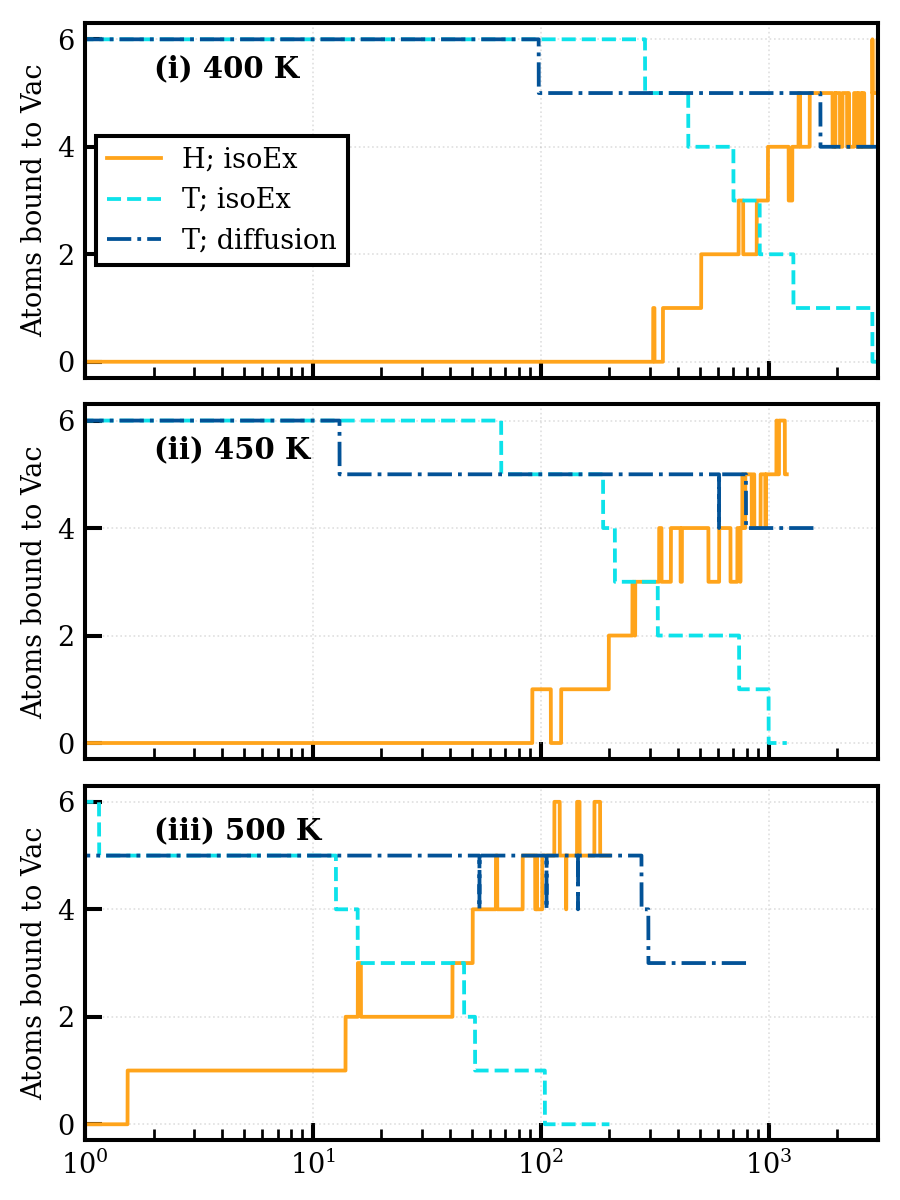
\includegraphics[width=0.99\textwidth]{1Vac_isoEx_HT_log.png}  
  \caption{Logarithmic time scale}
  %\label{fig:sub-first}
\end{subfigure}
\begin{subfigure}{.5\textwidth}
  \centering
  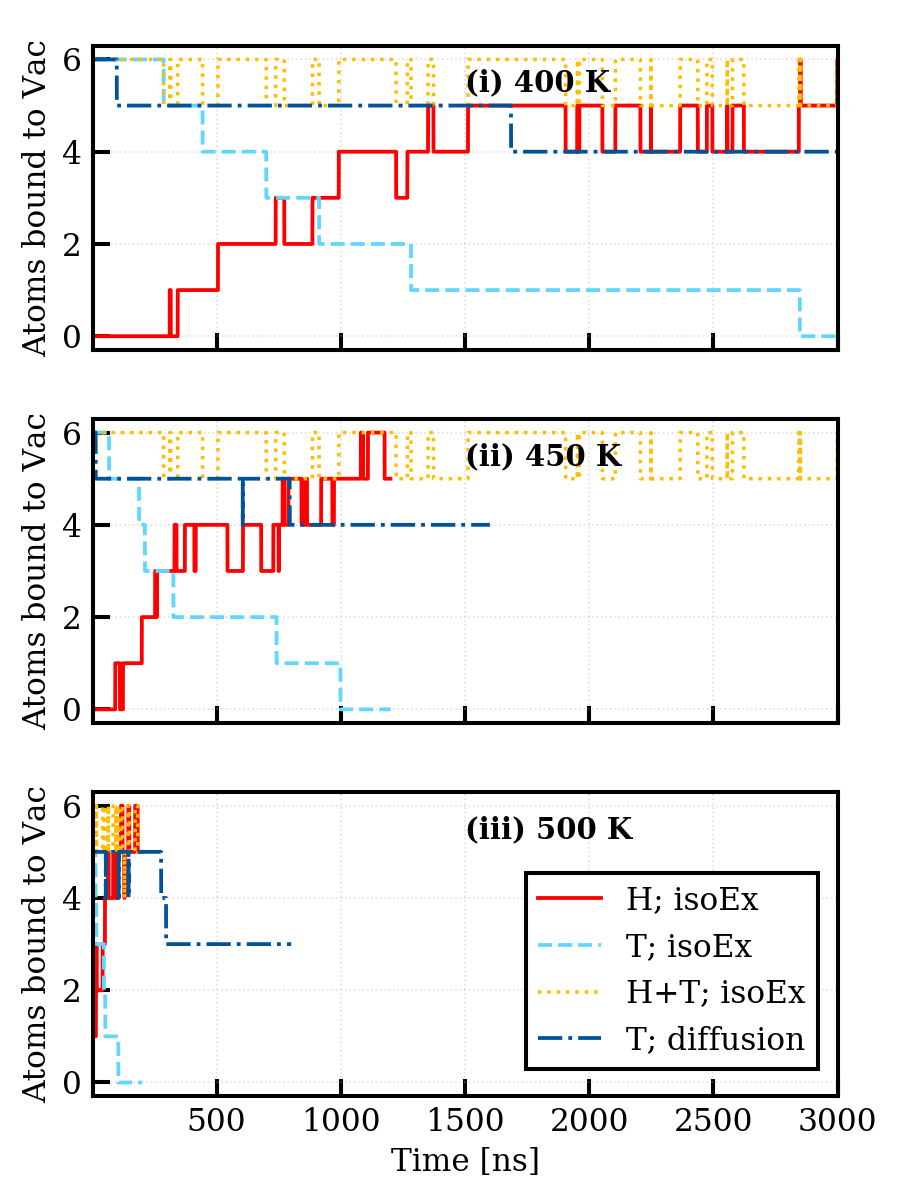
\includegraphics[width=0.99\textwidth]{1Vac_isoEx_HT.png}  
  \caption{Linear time scale}
  %\label{fig:sub-second}
\end{subfigure}
\caption{Number of H and T atoms bound to the monovacancy for isotope exchange and monoisotopic diffusion simulations}
 \label{Fig:1Vac_results} 
\end{figure}


\begin{figure}[!ht]
\begin{subfigure}{.5\textwidth}
  \centering
 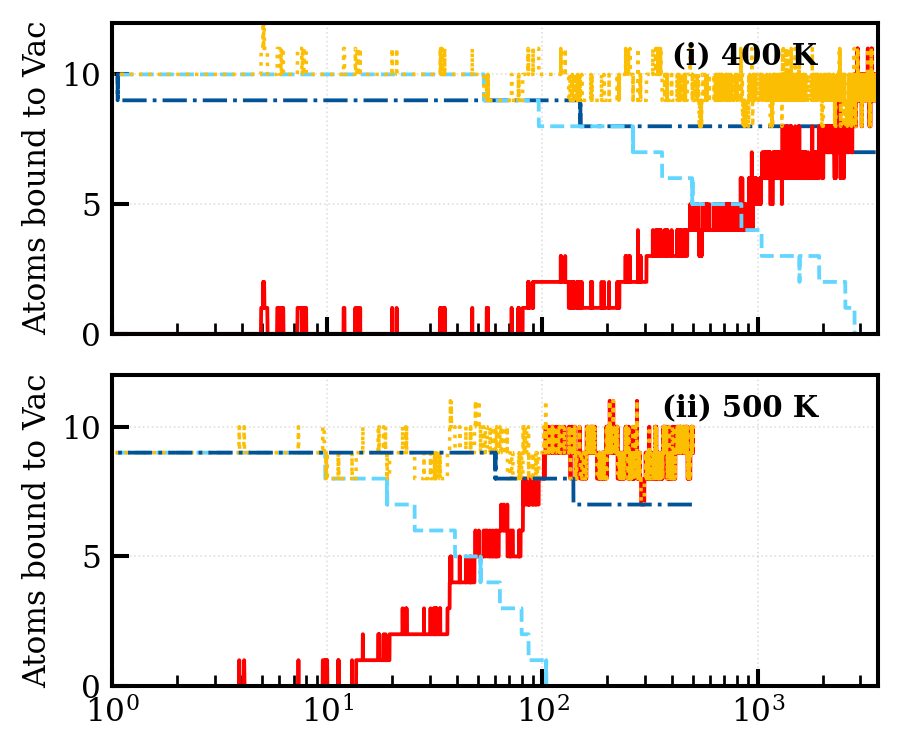
\includegraphics[width=0.99\textwidth]{2Vac_isoEx_HT_log.png}  
  \caption{Logarithmic time scale}
  %\label{fig:sub-first}
\end{subfigure}
\begin{subfigure}{.5\textwidth}
  \centering
  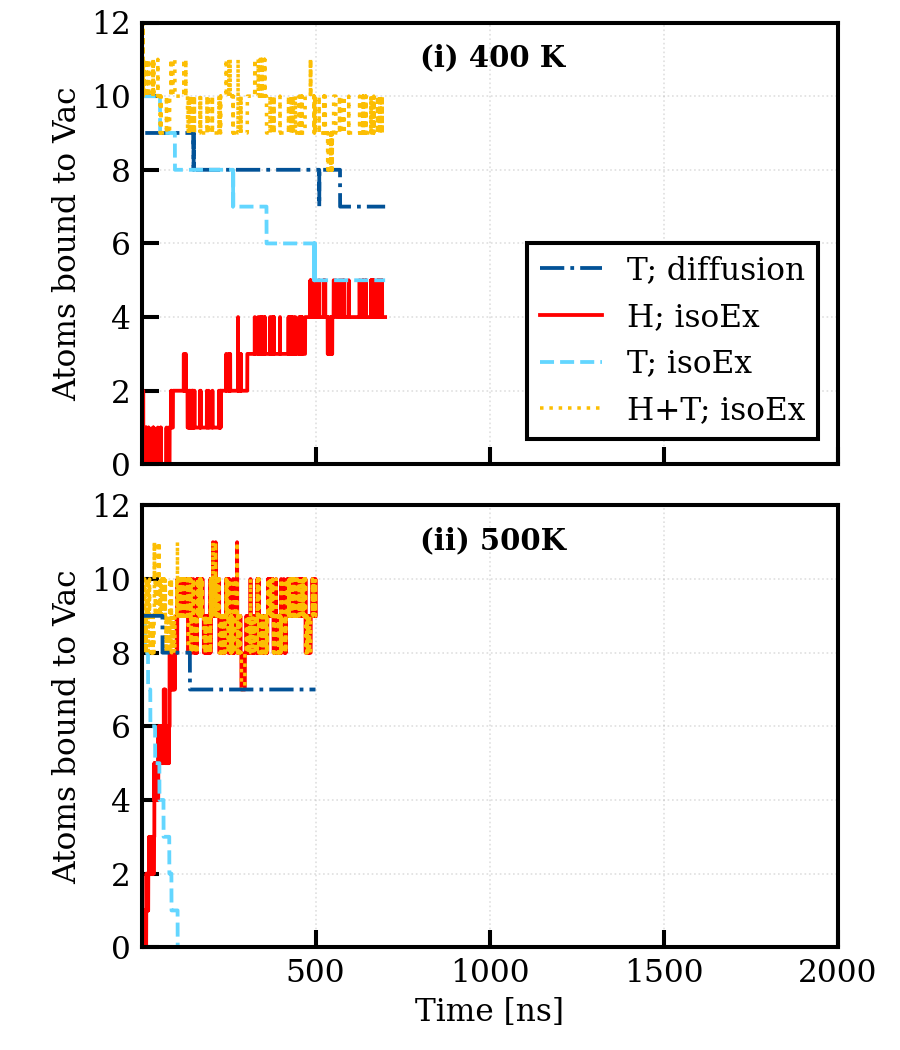
\includegraphics[width=0.99\textwidth]{2Vac_isoEx_HT.png}  
  \caption{Linear time scale}
  %\label{fig:sub-second}
\end{subfigure}
   \caption{Number of H and T atoms bound to the divacancy for isotope exchange and monoisotopic diffusion simulations}
   \label{Fig:2Vac_results} 
\end{figure}

Compared to DFT \cite{heinolaTungstenDFT}, the EAM potential used in this work gives slightly smaller binding energies for the hydrogen-vacancy interaction (Fig. \ref{Fig:Ebind1H_DFT}). 
Absolute tritium removal rates might thus not be directly comparable to experiments, whereas the relative differences between isotope exchange and vacuum annealing simulations are still valid.

Plotting the potential energy of the individual T atoms as a function of time as in Fig. \ref{Fig:Epot}, we can see sharp fluctuations as the atoms move around inside the defect, transitioning in and out of binding energy states.
This seemingly irrelevant fact shows on an atomic level what has been hypothesised based on macroscopic observations to be the basis of the isotope exchange mechanism.
We can also see from both Fig. \ref{Fig:1Vac_results} and \ref{Fig:2Vac_results} that the combined number of T and H in the defects are kept roughly constant during the isotope exchange simulations, with H atoms rapidly taking the place of detrapped T.

\begin{figure}[!ht]
\begin{subfigure}{.48\textwidth}
	\center
	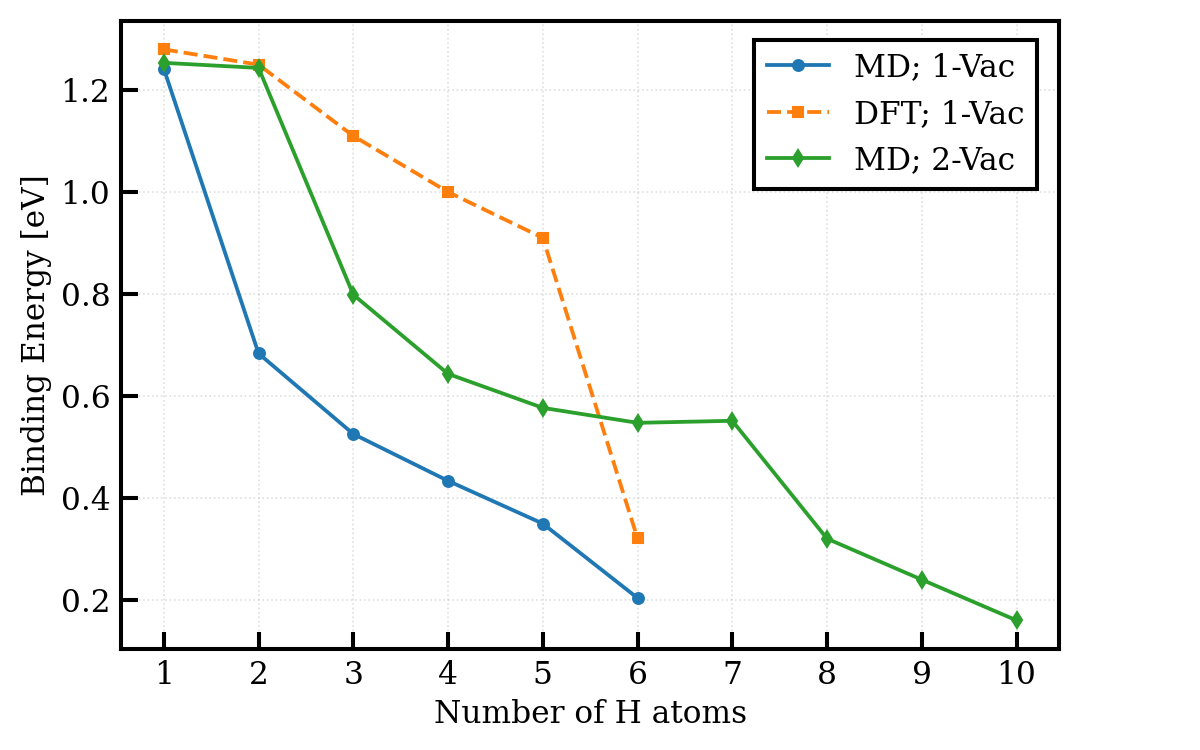
\includegraphics[width=1.1\linewidth]{Ebind.png}
	\caption{Comparision of the H-W binding energy in MD using the EAM1 potential by Bonny \textit{et. al} and DFT results by Heinola \textit{et. al. }\cite{heinolaTungstenDFT}}
	\label{Fig:Ebind1H_DFT}
\end{subfigure}
\hspace{3mm}
\begin{subfigure}{.48\textwidth}
	\center
	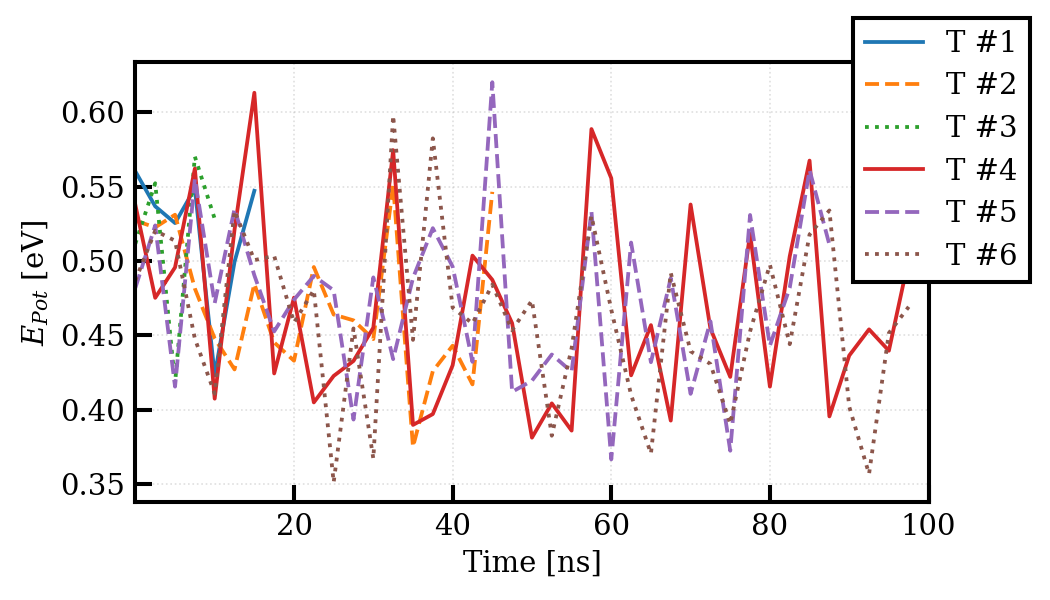
\includegraphics[width=1.1\linewidth]{epot.png}
	\caption{The potential energies of all individual T atoms in a 500 K simulation.\vspace*{6mm}}
	\label{Fig:Epot}
  %\label{fig:sub-second}
\end{subfigure}
\end{figure}


% ----------------------------------------------------------------------------------
\section{Dislocations}
% ----------------------------------------------------------------------------------
The dislocation results are shown in Fig. \ref{Fig:disloc_results} and indicate an enhanced T-removal rate when utilising isotope exchange at 500 K. 
At 400 K, on the other hand, there is no significant difference between the two methods.

Due to the extremely long simulation that would have been required for complete T-removal using the monoisotopic method even at 500 K, we can only state that removal using isotope exchange appears to be several orders of magnitude faster.
 

\begin{figure}[!ht]
\begin{subfigure}{.5\textwidth}
  \centering
 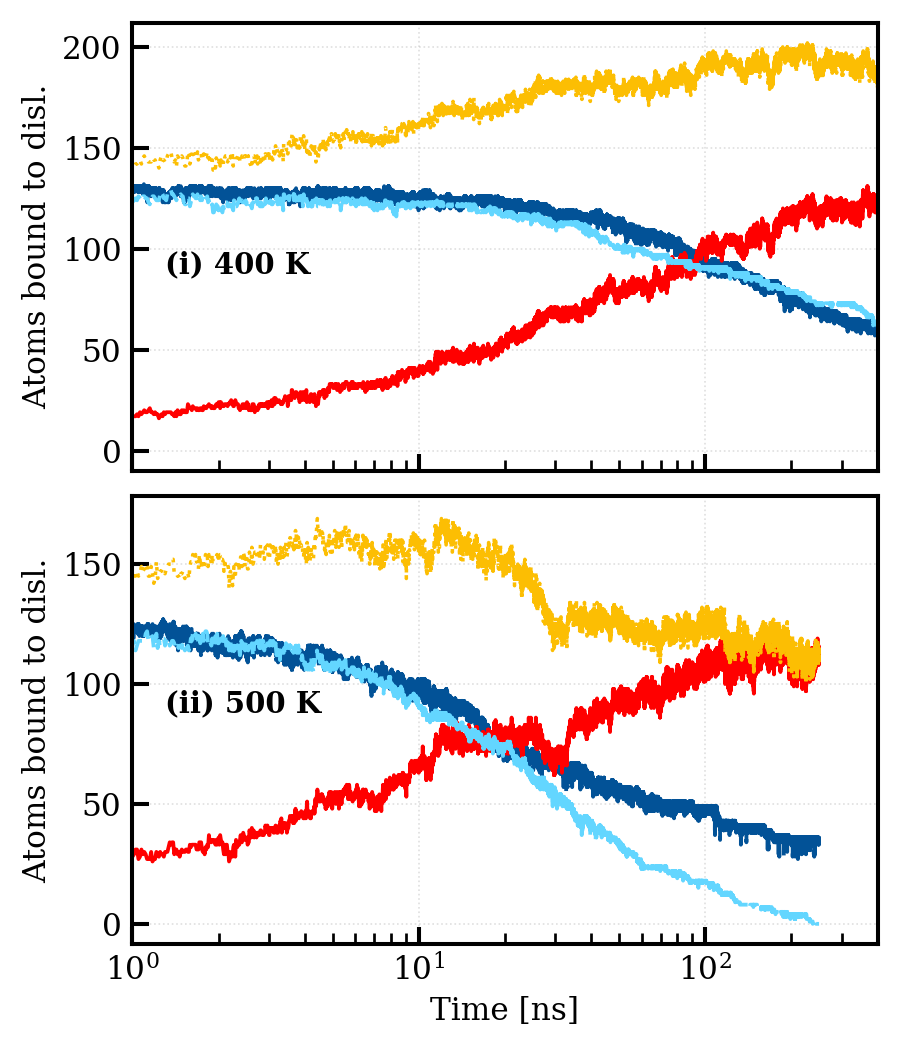
\includegraphics[width=0.99\textwidth]{disloc_isoEx_HT_log.png}  
  \caption{Logarithmic time scale}
  %\label{fig:sub-first}
\end{subfigure}
\begin{subfigure}{.5\textwidth}
  \centering
  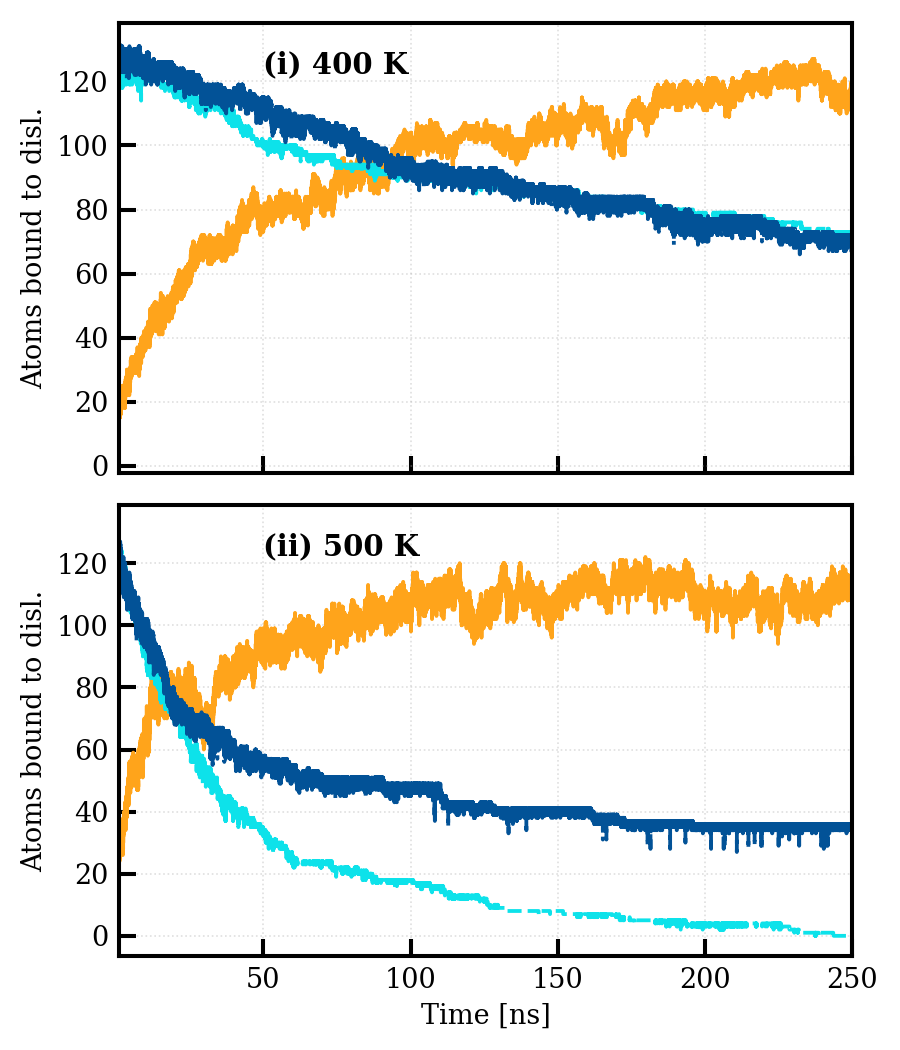
\includegraphics[width=0.99\textwidth]{disloc_isoEx_HT.png}  
  \caption{Linear time scale}
  %\label{fig:sub-second}
\end{subfigure}
   \caption{Number of H and T atoms bound to the dislocation for isotope exchange and monoisotopic diffusion simulations}
   \label{Fig:disloc_results} 
\end{figure}



% ----------------------------------------------------------------------------------
\section{Grain boundaries}
% ----------------------------------------------------------------------------------
The grain boundary results are shown in Fig. \ref{Fig:GB_results}. 
Here, as was the case with the dislocation, an improved T-removal rate can only be observed at 500 K.
Similarly, the exact difference in removal rate was difficult to determine without excessive use of computing resources, but can be clearly seen from Fig. \ref{Fig:GB_results} to be several orders of magnitude higher for the isotope exchange simulations.
The shape of the 


\begin{figure}[!ht]
\begin{subfigure}{.5\textwidth}
  \centering
 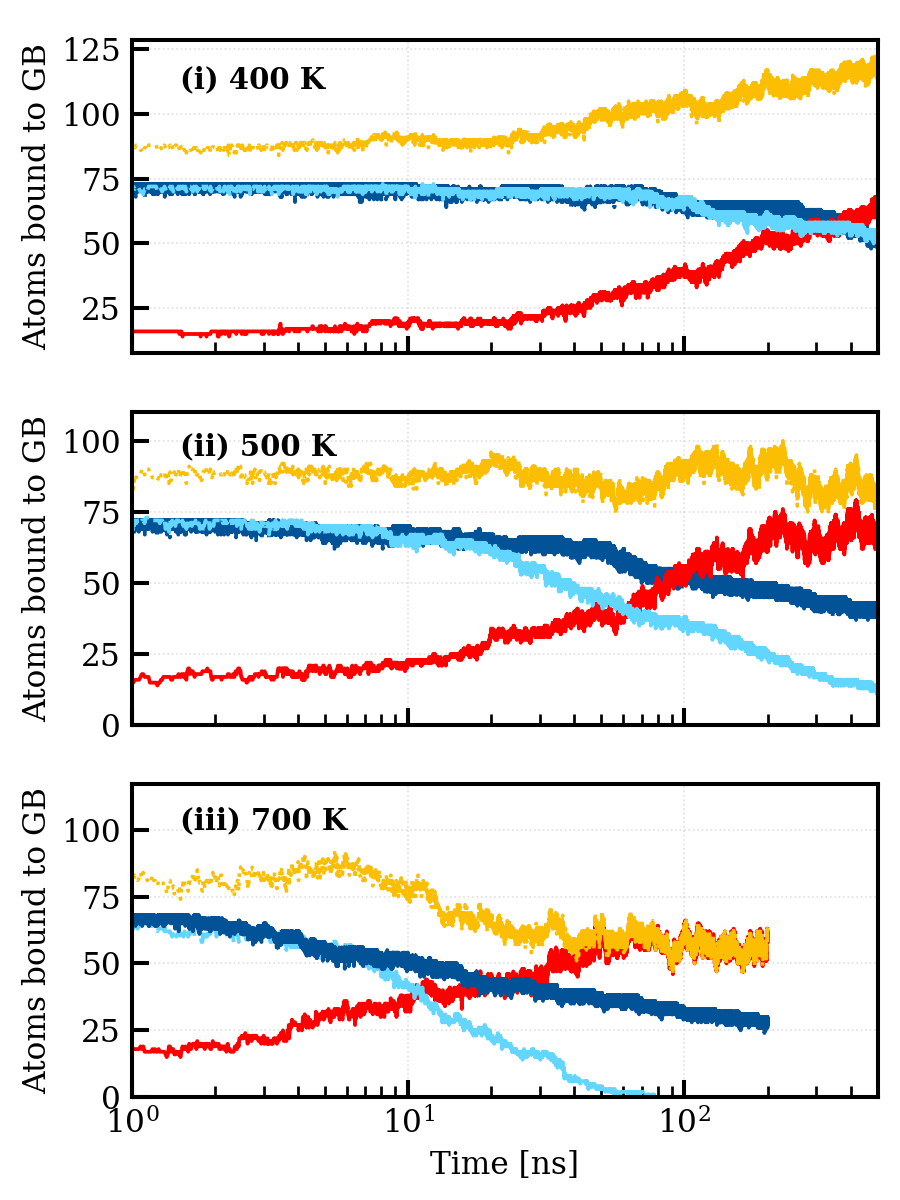
\includegraphics[width=0.99\textwidth]{GB_isoEx_HT_log.png}  
  \caption{Logarithmic time scale}
  %\label{fig:sub-first}
\end{subfigure}
\begin{subfigure}{.5\textwidth}
  \centering
  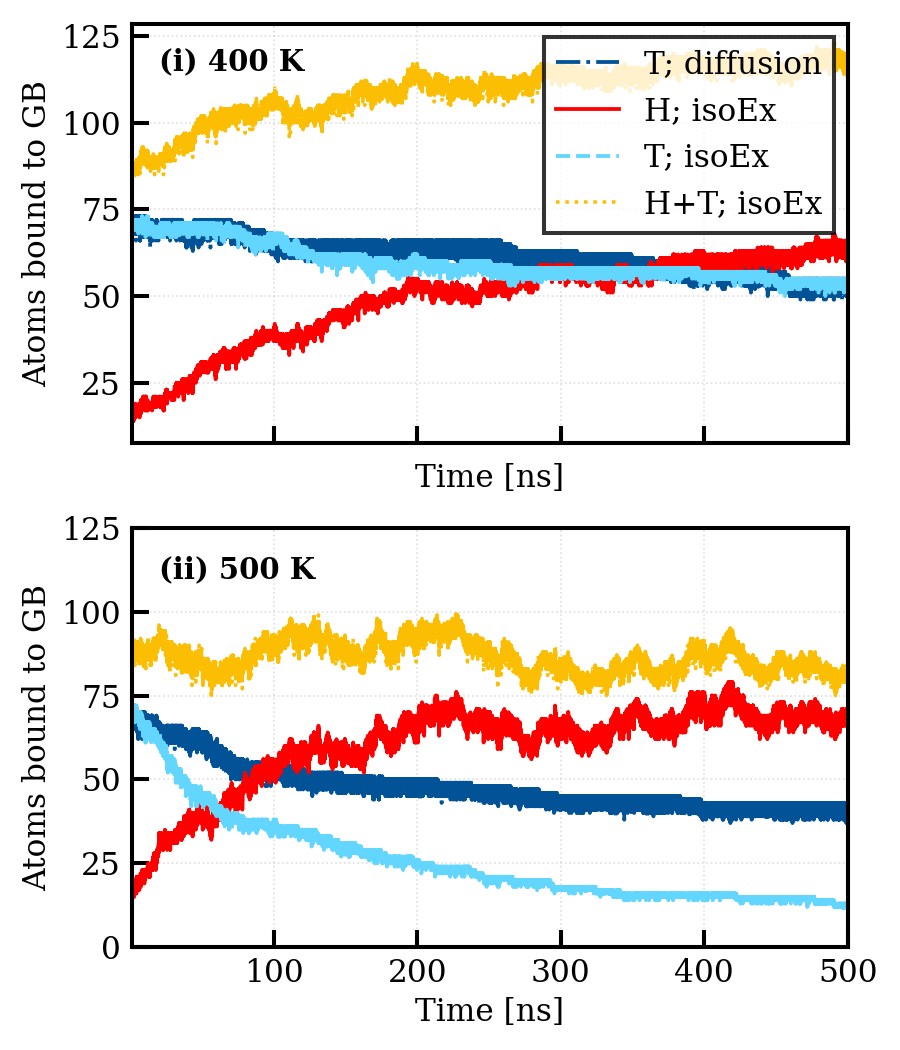
\includegraphics[width=0.99\textwidth]{GB_isoEx_HT.png}  
  \caption{Linear time scale}
  %\label{fig:sub-second}
\end{subfigure}
   \caption{Number of H and T atoms bound to the grain boundary for isotope exchange and monoisotopic diffusion simulations}
   \label{Fig:GB_results} 
\end{figure}

